\section{Classification of Particles as Closure Structures}
\label{sec:particles}

\subsection{Reformulating Particle Identity}

In conventional particle physics, particles are treated as fundamental entities
belonging to distinct categories.
Within the present framework, particles are interpreted as stable configurations
of closure structure:
\begin{equation}
  \boxed{
    \text{What is observed as a particle corresponds to a class of
    stable closure configurations.}
  }
\end{equation}
Particle classification is therefore reformulated as a classification
of closure geometry.

\subsection{Degeneracy as the Organizing Principle}

Section~\ref{sec:triangular} established that triangular closure admits
different structural regimes depending on degeneracy.
This provides a natural organizing principle:
\begin{equation}
  \boxed{\text{Particle type is determined by the degree of triangular degeneracy.}}
\end{equation}
Degeneracy controls the number of effective degrees of freedom,
the symmetry structure, and the stability characteristics of each configuration.

\subsection{Three Structural Regimes}

\paragraph{Non-degenerate triangular closure.}
Finite area, three independent directions, maximal internal coupling.
\begin{equation}
  \boxed{
    \text{Non-degenerate closure represents the maximally articulated}
    \quad
    \text{configuration within the triangular regime.}
  }
\end{equation}

\paragraph{Degenerate triangular closure.}
Area approaches zero, one direction collapses, two effective degrees of freedom remain.
\begin{equation}
  \boxed{\text{Degenerate closure represents a reduced structural configuration.}}
\end{equation}

\paragraph{Extreme degeneracy.}
Area effectively vanishes, structure collapses toward a point,
minimal internal interaction.
\begin{equation}
  \boxed{\text{Extreme degeneracy corresponds to minimal closure structure.}}
\end{equation}

\subsection{Structural Interpretation of Particle Types}

These three regimes map to familiar particle classes,
as summarized in Table~\ref{tab:particles} and Fig.~\ref{fig:particles}.

\begin{table}[h]
  \centering
  \begin{tabular}{ll}
    \toprule
    Closure regime & Structural interpretation \\
    \midrule
    Non-degenerate triangle & baryon-like structures \\
    Degenerate triangle     & lepton-like structures \\
    Extreme degeneracy      & neutrino-like structures \\
    \bottomrule
  \end{tabular}
  \caption{
    Correspondence between closure regimes and particle classes.
    This mapping is structural rather than identificational.
  }
  \label{tab:particles}
\end{table}

\begin{equation}
  \boxed{\text{Particle classes correspond to geometric regimes of closure.}}
\end{equation}

\begin{figure}[h]
  \centering
  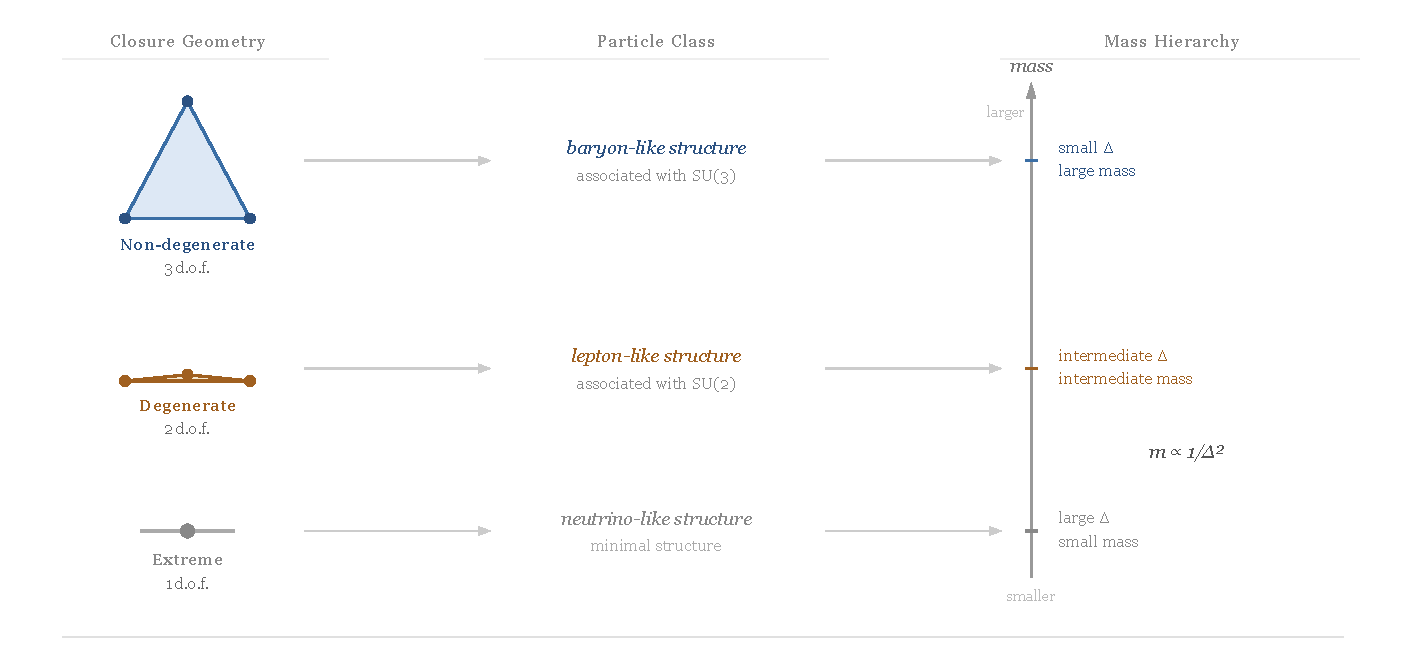
\includegraphics[width=\textwidth]{figures/VED_Vol2_Figure3.pdf}
  \caption{
    Particle classes as closure geometry.
    Triangular closure admits three structural regimes depending on degeneracy.
    These regimes correspond to baryon-like, lepton-like, and neutrino-like structures.
    Mass is associated with distance from the complete-closure limit,
    with $m \propto 1/\Delta^2$.
  }
  \label{fig:particles}
\end{figure}

\subsection{The Degeneracy Ladder}

The three regimes form a continuous hierarchy:
\begin{equation}
  \text{non-degenerate} \;\rightarrow\; \text{degenerate} \;\rightarrow\; \text{extreme.}
\end{equation}
\begin{equation}
  \boxed{\text{Particles form a hierarchy along a degeneracy continuum.}}
\end{equation}
Discrete particle types can be viewed as stable points along this continuous structure.

\subsection{Mass as Distance from Closure}

Define the closure deficit relative to the complete-closure limit:
\begin{equation}
  \Delta_k = L_{\max} - L_k.
\end{equation}
Mass scales as:
\begin{equation}
  \label{eq:mass}
  m \propto \frac{1}{\Delta_k^2}.
\end{equation}
Stronger closure implies smaller $\Delta$ and larger mass;
weaker closure implies larger $\Delta$ and smaller mass.
\begin{equation}
  \boxed{\text{Mass can be interpreted as distance from the closure limit.}}
\end{equation}

Here the complete-closure limit is not assumed to be an attainable physical
state.
It is a limiting representation of the point at which the internal differences
required for persistent structure would disappear.

\subsection{Discrete Particles from Continuous Geometry}

Although closure geometry varies continuously, observed particles appear discrete:
\begin{equation}
  \boxed{
    \text{Discrete particles correspond to stable points within a
    continuous geometric landscape.}
  }
\end{equation}
Particle classification is not a taxonomy of independent entities,
but a discretization of underlying structure.
